The most recent gantt chart created is significantly different than the original gantt chart for the semester, as the initial gantt chart assumed everything would be finished with the design process and only printing and implementation needed to be completed. Within the first week, however, it was decided that the differential gearboxes used in the shoulder and wrist were not precise enough to be used in the design, so alternate solutions were sought. A design for a harmonic gearbox was chosen and tested, and was found to be useful for both torque and accuracy of the manipulator. Because of the change in gearboxes, the design of the manipulator had to be changed, and software writing was pushed back until the design was finalized. The shoulder link with the harmonic gearbox design printed in the fourth week, so construction and implementation of the shoulder joint with the servos was able to be worked on. During this week, it was also decided that MX-64T servos would be used instead of the MX-12W servos, as the MX-64T servos increased torque output and were available within the robotics lab. During the fourth week writing to the servos also presented some issues, as occasionally the servos would do exactly one too few rotations, so software had to be pushed back again. In the next week, a harmonic gearbox with a lower gear ratio was designed and printed, and after successful implementation with the MX-64T servos the new gearbox was chosen to be placed in the three spherical wrist joints, causing another redesign. With the shoulder and elbow joints printed and assembled, software was able to progress, which describes the last changes and progress made on the gantt chart before spring break. The last Gantt chart can be seen on the following page.
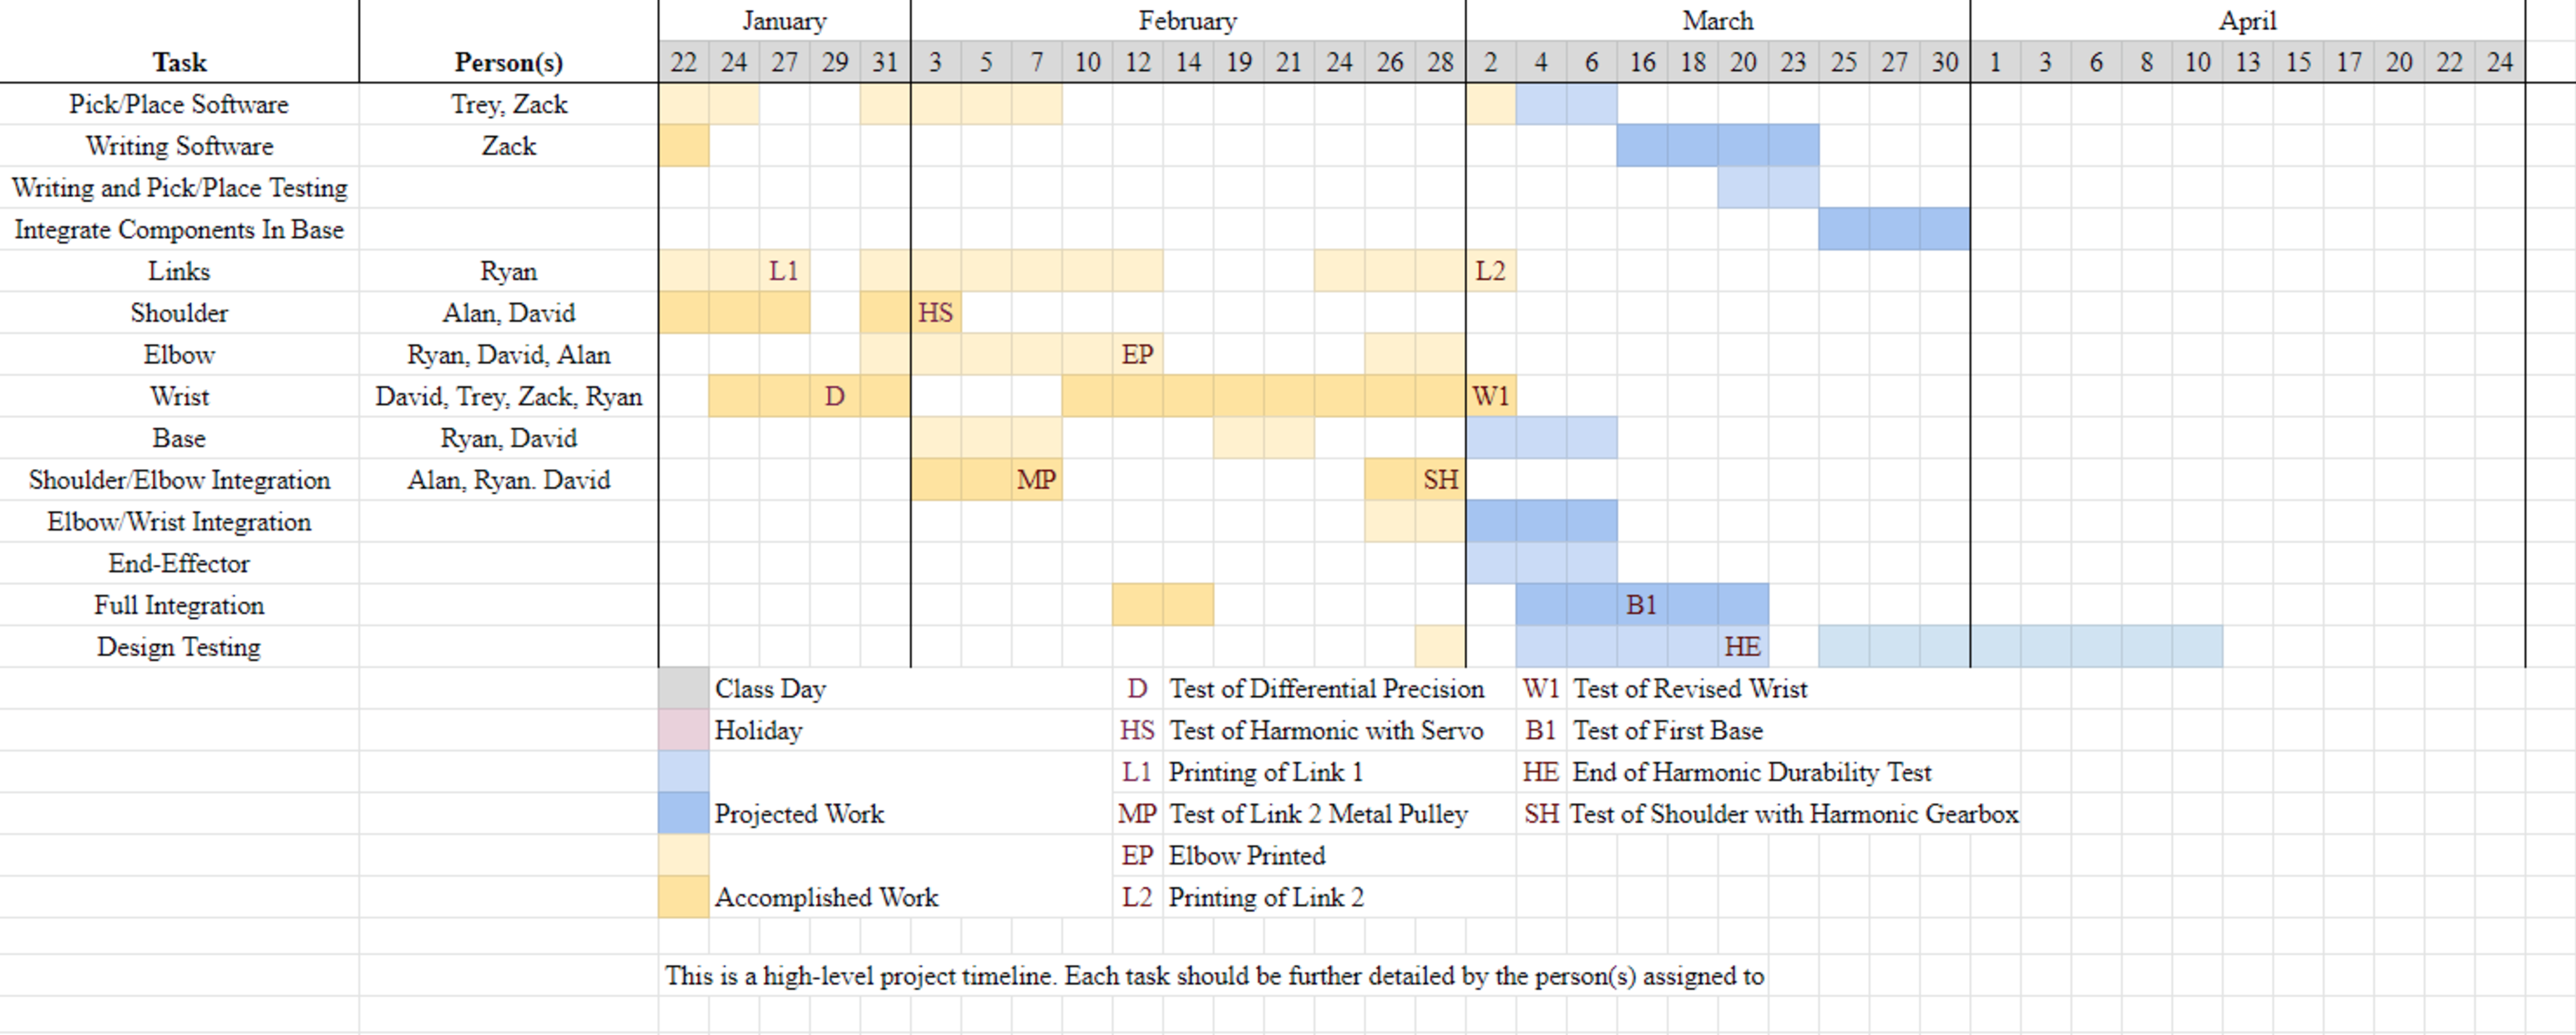
\includepdf[landscape,pages=-]{gantt2}
Overall, most of the changes to the gantt chart were due to the redesign process, where printing pieces and finding issues with the each component prompted slight redesigns and reprinting, the process of which tended to take a full two days between class periods before the new components could be used and potentially redesigned again if there were other problems that arose. In January and early February, the redesign process only took a day or two, but in late February the Rapid Prototype Lab started to receive more print requests from other capstone teams so the redesign process started to take longer, from three or four days up to a week. This wait time created most of the delays, as waiting for new parts to print delayed both implementation and general design progression.

For the project budget, the MEIOSIS team stayed within the \$800 budget allowed by the engineering department, and the bill of material is shown in Table \ref{tab:bom3}.
\begin{table}[htp]
  \center
  \caption{MEIOSIS Bill of Materials with Costs}
  \label{tab:bom3}
\begin{tabular}{c|c|c|C{3cm}|c}
Part & Qty & Individual price & Transaction Cost & MEIOSIS Cost \\\hline
M3x30mm Screws & 2 & \$5.99 & \$11.98 & \$11.98 \\
M3 Locking nuts & 1 & \$7.99 & \$7.99 & \$7.99 \\
TRiREAK AC Bearing & 7 & \$9.00 & \$63.00 & \$63.00 \\
Thrust Bearing & 1 & \$7.99 & \$7.99 & \$7.99 \\
Skateboard Bearings & 1 & \$5.29 & \$5.29 & \$5.29 \\
MX-64T Servo & 3 & \$299.90 & \$899.70 & \$0 \\
MX-12W Servo & 3 & \$65.90 & \$197.70 & \$197.70 \\
AX-12A Servo* & 1 & \$44.90 & \$44.90 & \$44.90 \\
Raspberry Pi 3B & 1 & \$34.95 & \$34.95 & \$34.95 \\
RPi Power Supply & 1 & \$9.95 & \$9.95 & \$9.95 \\
SD Card & 1 & \$12.95 & \$12.95 & \$12.95 \\
U2D2 & 1 & \$49.90 & \$49.90 & \$0 \\
MX/RX Power Hub & 1 & \$7.95 & \$7.95 & \$0 \\
RPS-200-12-C* & 1 & \$56.55 & \$56.55 & \$56.55 \\
DC Male Barrel Cable* & 1 & \$1.24 & \$1.24 & \$1.24 \\
Hatchbox PLA & 2 Spools & \$19.99/Spool & \$39.98 & \$0 \\
Shipping/Tax & N/A & N/A & \$7.95 & \$7.95 \\
Discounts & N/A & N/A & -\$8.17 & -\$8.17 \\
& & \textbf{Total Cost} & \$1,451.80 & \$454.27 \\
\end{tabular}
\end{table}

From Table \ref{tab:bom3}, the total spent by MEIOSIS is \$454.27, below the \$800 allocated to the team. The total cost of the manipulator if all items needed to be purchased came out to \$1,451.80, with a majority of the cost being the MX-64T servos. The amount of PLA required for the manipulator came out to between one and two kilograms of material, so the price of two 1kg spools of PLA is listed in the table.
\newpage
